% !TeX program = pdflatex
% Build: latexmk -pdf mainv1.tex (replace with this file's name).
\documentclass[a4paper,11pt]{article}
\usepackage{jheppub}
\usepackage{mathtools,bm}
\usepackage{orcidlink}
\allowdisplaybreaks[1]

% General-purpose commands from the FEC manuscripts.
% physics supplies bra, ket, braket, dyad, matrixel, expval,
% abs, norm, comm, acomm, dv, pdv, dd, and trace commands.
\usepackage{physics}
% Keep \sec for the trigonometric function and \pb for Poisson brackets.
\newcommand{\secref}[1]{Sec.~\ref{#1}}
\newcommand{\fig}[1]{Fig.~\ref{#1}}
\newcommand{\figs}[2]{Figs.~\ref{#1} and~\ref{#2}}
\newcommand{\eq}[1]{Eq.~\eqref{#1}}
\newcommand{\eqs}[2]{Eqs.~\eqref{#1} and~\eqref{#2}}
\newcommand{\eqss}[3]{Eqs.~\eqref{#1}~\eqref{#2} and~\eqref{#3}}
\newcommand{\refcite}[1]{Ref.~\cite{#1}}
\newcommand{\refs}[1]{Refs.~\cite{#1}}
\newcommand*{\Scale}[2][4]{\scalebox{#1}{\ensuremath{#2}}}

\newcommand{\pp}[1]{\left(#1\right)}
\newcommand{\bb}[1]{\left[#1\right]}
\newcommand{\cc}[1]{\left\{#1\right\}}
\newcommand{\vv}[1]{\left\langle #1 \right\rangle}
\newcommand{\bigpp}[1]{\big(#1\big)}
\newcommand{\bigbb}[1]{\big[#1\big]}
\newcommand{\bigcc}[1]{\big\{#1\big\}}
\newcommand{\bigvv}[1]{\big\langle #1 \big\rangle}
\newcommand{\Bigpp}[1]{\Big(#1\Big)}
\newcommand{\Bigbb}[1]{\Big[#1\Big]}
\newcommand{\Bigcc}[1]{\Big\{#1\Big\}}
\newcommand{\Bigvv}[1]{\Big\langle #1 \Big\rangle}
\newcommand{\biggpp}[1]{\bigg(#1\bigg)}
\newcommand{\biggbb}[1]{\bigg[#1\bigg]}
\newcommand{\biggcc}[1]{\bigg\{#1\bigg\}}
\newcommand{\biggvv}[1]{\bigg\langle #1 \bigg\rangle}

\newcommand{\iv}[1]{\left[#1\right]}
\newcommand{\bigiv}[1]{\big[#1\big]}
\newcommand{\biggiv}[1]{\bigg[#1\bigg]}

\newcommand{\beq}[1][]{\begin{equation}\if\relax\detokenize{#1}\relax\else\label{#1}\fi}
\newcommand{\eeq}{\end{equation}}
\newcommand{\bse}[1][]{\begin{subequations}\if\relax\detokenize{#1}\relax\else\label{#1}\fi}
\newcommand{\ese}{\end{subequations}}
\newcommand{\nn}{\nonumber}

\newcommand{\wt}[1]{\widetilde{#1}}
\newcommand{\GeV}{\mathrm{GeV}}
\newcommand{\pbu}{\mathrm{pb}}
\newcommand{\MS}{\overline{\mathrm{MS}}}
\newcommand{\LQCD}{\Lambda_{\mathrm{QCD}}}
\newcommand{\lo}{{[0]}}
\newcommand{\nlo}{{[1]}}

% Add your own macros here.

\title{Calculation with Spins}
\author{Shu-Tao Zhang\,\orcidlink{0009-0009-5269-2364}}
\affiliation{School of Physics, Peking University, Beijing 100871, China}
\emailAdd{shutaozhang@pku.edu.cn}
\date{\today}
\abstract{%
% State the question, approach, main result, and domain of validity.
Write your abstract here.
}

\begin{document}
\maketitle
\flushbottom

\section{Setup and conventions}
\label{sec:setup}
% Define the observable, conventions, scales, and assumptions.
In this note, we calculate the helicity amplitudes for the process $e^+ e^- \to \mu^+ \mu^-$, including the effects of transverse spin polarization. We adopt the spinor helicity formalism and follow the conventions outlined in Peskin book. 
The kinematics are summarized as follows, the incoming electron and positron have momenta $p_1$ and $p_2$, respectively, while the outgoing muon and antimuon have momenta $k_1$ and $k_2$. The explicit expressions for the momentum are given by:
\begin{align}
    p_1^\mu &= \frac{\sqrt{s}}{2} (1, 0, 0, 1), \\
    p_2^\mu &= \frac{\sqrt{s}}{2} (1, 0, 0, -1), \\
    k_1^\mu &= \frac{\sqrt{s}}{2} (1, \sin\theta, 0, \cos\theta), \\
    k_2^\mu &= \frac{\sqrt{s}}{2} (1, -\sin\theta, 0, -\cos\theta),
\end{align}
While the Mandelstam variables are defined as:
\begin{align}
    s &= (p_1 + p_2)^2, \\
    t &= (p_1 - k_1)^2 = \frac{s}{2}\pp{\cos\theta-1}, \\
    u &= (p_1 - k_2)^2 = \frac{s}{2}\pp{-\cos\theta-1},
\end{align}
with $s + t + u = 0$ in our massless approximation.

{\emph{helicity conventions ---}}
Now we define the spinor helicity conventions. For simplicity we consider the massless case, while the massive case can be left as future investigation.
In the Appendix B of Peskin book, the spinors are:
\begin{align}
    u_\lambda(p) &= \begin{pmatrix} \sqrt{p\cdot\sigma} \, \xi_\lambda \\ \sqrt{p\cdot\bar{\sigma}} \, \xi_\lambda \end{pmatrix}, \\
    v_\lambda(p) &= \begin{pmatrix} \sqrt{p\cdot\sigma} \, \eta_\lambda \\ -\sqrt{p\cdot\bar{\sigma}} \, \eta_\lambda \end{pmatrix},
\end{align}
With the spinors $\xi_\lambda$ and $\eta_\lambda$ defined in Eq.~(3.134)
\begin{align}
    \xi_+(p) &= \begin{pmatrix} \cos\frac{\theta}{2} \\ e^{i\phi}\sin\frac{\theta}{2} \end{pmatrix}, \nn\\
    \xi_-(p) &= \begin{pmatrix} -e^{-i\phi}\sin\frac{\theta}{2} \\ \cos\frac{\theta}{2} \end{pmatrix}, \nn\\
    \eta_+(p) &= \xi_-(p),  \nn\\
    \eta_-(p) &= -\xi_+(p),
\end{align}
which lead to
\begin{align}
    u_\pm(p) &= \begin{pmatrix} \sqrt{E \mp \abs{\bm p}} \, \xi_\pm \\ \sqrt{E \pm \abs{\bm p}} \, \xi_\pm \end{pmatrix}, \\
    v_\pm(p) &= \begin{pmatrix} \sqrt{E \pm \abs{\bm p}} \, \eta_\pm \\ -\sqrt{E \mp \abs{\bm p}} \, \eta_\pm \end{pmatrix}.
\end{align}
Here $\theta$ and $\phi$ are the polar and azimuthal angles of the momentum $p$ in the spherical coordinate system, which should be separated from the kinematics.
The helicity basis here means the spin is aligned with the momentum direction, while in the traditional conventions, including Appendix B in Peskin book, the spin is aligned with the $z$-axis.

One should note that the spinor helicity allow an overall arbitrary phase. However, during the calculation, one should fix the phase convention to avoid ambiguity for defining the transverse spin.
% For the fermion spinors $u$, one have a natural helicity operator definition, which is
% \begin{align}
    
% \end{align}

Finally, we demonstrate the relation of the spinor helicity and the chirality.
\begin{align}
    P_R u_+(p) &= u_+(p), \quad P_L u_-(p) = u_-(p), \quad \gamma_5 u_{L/R}(p) = \mp u_{L/R}(p), \\
    P_R v_-(p) &= v_-(p), \quad P_L v_+(p) = v_+(p), \quad \gamma_5 v_{L/R}(p) = \mp v_{L/R}(p).
\end{align}

\emph{transverse spin of fermion ---}
The derivation of the transverse spin of a fermion can be found in hep-ph/0104283, Eq.~(2.2.6). Normally we don't use the transverse polarized spinor directly, still, we summarize the main results here.
\begin{align}
    u^x_+(p) &= \frac{1}{\sqrt{2}}\bb{u_+(p) + u_-(p)}, \\
    u^x_-(p) &= \frac{1}{\sqrt{2}}\bb{u_+(p) - u_-(p)}, \\
    u^y_+(p) &= \frac{1}{\sqrt{2}}\bb{u_+(p) + i u_-(p)}, \\
    u^y_-(p) &= \frac{1}{\sqrt{2}}\bb{u_+(p) - i u_-(p)}, \\
    v^x_+(p) &= \frac{1}{\sqrt{2}}\bb{v_+(p) + v_-(p)}, \\
    v^x_-(p) &= \frac{1}{\sqrt{2}}\bb{v_+(p) - v_-(p)}, \\
    v^y_+(p) &= \frac{1}{\sqrt{2}}\bb{v_+(p) - i v_-(p)}, \\
    v^y_-(p) &= \frac{1}{\sqrt{2}}\bb{v_+(p) + i v_-(p)}.
\end{align}
The last two equations comes from the fact that charge conjugation involves a conjugation of the spinor, which flips the sign of the imaginary unit $i$.
Please note that all these component allows an overall arbitrary phase, what is important is the relative phase of $u_+$ and $u_-$.
Therefore, in some other references, one may find different overall phase conventions, don't be surprised.

A more convenient way to think about the transverse spin is to use the density matrix formalism, which is discussed in hep-ph/0104283, Eq.~(2.3.4). The density matrix of a fermion with transverse spin can be expressed as:
\begin{align}
    \rho = \tfrac 1 2 \begin{pmatrix}
        1+s_z \quad s_x-is_y\\
        s_x+is_y \quad 1-s_z
    \end{pmatrix}
    \propto \mathcal{H}_{\lambda\lambda'} = \begin{pmatrix}
        \mathcal{H}_{++} \quad \mathcal{H}_{+-}\\
        \mathcal{H}_{-+} \quad \mathcal{H}_{--}
    \end{pmatrix},
\end{align}
where the $\mathcal{H}_{\lambda\lambda'}$ is the interference term of the helicity amplitudes, with the observed fermion spin indices open.
In this expression, the overall phase in the transverse polarized spinor is irrelevant, however, the relative phase between $u_+$ and $u_-$ still counts. For example, if we add a phase factor $e^{i\bar\phi}$ to $u_+$, then the density matrix becomes:
\begin{align}
    \rho = \tfrac 1 2 \begin{pmatrix}
        1+s_z \qquad e^{-i\bar\phi}(s_x-is_y)\\
        e^{i\bar\phi}(s_x+is_y) \qquad 1-s_z
    \end{pmatrix}.
\end{align}

Finally, one can calculate

\section{Derivation}
\label{sec:derivation}
% Derive the result and explain the approximations.
In this section, we calculate the helicity amplitudes for the process $e^+ e^- \to \mu^+ \mu^-$, which is an easy example for the future calculation.
Though many much more effective methods exist, we use the easiest one. We first write down the explicit expressions for the spinors, then we substitute them into the Feynman ampltiudes.

% --------------- Feynman Diagram ---------------
\begin{figure}[htbp]
    \centering
    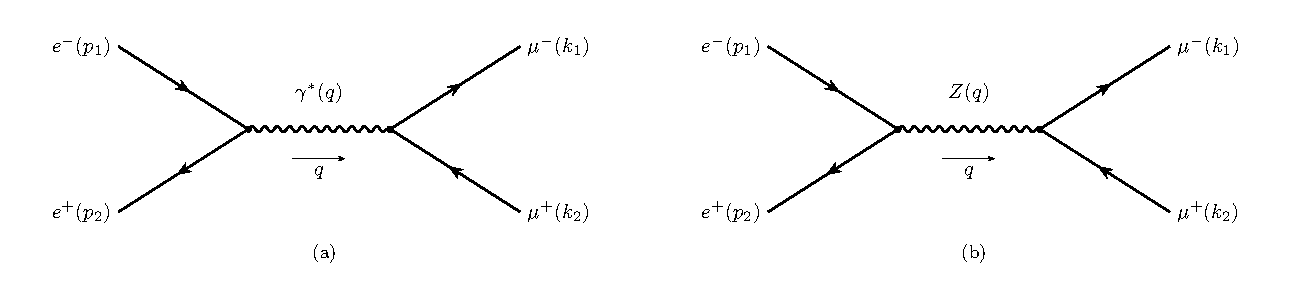
\includegraphics[width=\textwidth]{ee_to_mumu_tree.pdf}
    \caption{Feynman diagrams involving QED and EW interactions}
    \label{fig:feynman-diagrams}
\end{figure}
% ---------------

Consider the QED process first and leave all the helicity indices open, we get:
\begin{align}
    i\mathcal{M}_{\lambda_1\lambda_2\lambda_3\lambda_4} &= \bar{v}_{\lambda_2}(p_2) (-ie\gamma^\mu) u_{\lambda_1}(p_1) \frac{-i g_{\mu\nu}}{s} \bar{u}_{\lambda_3}(k_1) (-ie\gamma^\nu) v_{\lambda_4}(k_2).
\end{align}

Substituting the explicit massless spinors gives the helicity amplitudes below.
To fix their relative phases, we use the two-component spinors defined above and choose the polar and azimuthal angles
\begin{align}
    (\theta_{p_1},\phi_{p_1}) &= (0,0), &
    (\theta_{p_2},\phi_{p_2}) &= (\pi,\pi), \nn\\
    (\theta_{k_1},\phi_{k_1}) &= (\theta,0), &
    (\theta_{k_2},\phi_{k_2}) &= (\pi-\theta,\pi).
\end{align}
The azimuth at the south pole is a spinor phase convention, even though it does not affect the momentum.
With rows labeled by $(\lambda_1,\lambda_2)$ and columns by $(\lambda_3,\lambda_4)$, the entries are $\mathcal{M}_{\lambda_1\lambda_2\lambda_3\lambda_4}/e^2$, rather than $i\mathcal{M}/e^2$:
\begin{equation}
\label{eq:qed-helicity-amplitudes}
    \begin{array}{c|cccc}
        (\lambda_1,\lambda_2)\backslash(\lambda_3,\lambda_4)
            & ++ & +- & -+ & -- \\ \hline
        ++  & 0 & 0 & 0 & 0 \\
        +-  & 0 & -(1+\cos\theta) & 1-\cos\theta & 0 \\
        -+  & 0 & 1-\cos\theta & -(1+\cos\theta) & 0 \\
        --  & 0 & 0 & 0 & 0
    \end{array}.
\end{equation}
Only opposite-helicity fermion--antifermion pairs contribute in the massless limit.
Summing over final helicities and averaging over initial helicities reproduces the unpolarized QED result,
\begin{equation}
\label{eq:qed-helicity-spin-sum}
    \frac{1}{4}\sum_{\lambda_1,\lambda_2,\lambda_3,\lambda_4}
    \left|\mathcal{M}_{\lambda_1\lambda_2\lambda_3\lambda_4}\right|^2
    = e^4\left(1+\cos^2\theta\right),
\end{equation}
which also agrees with an independent Dirac-trace calculation.

\section{Results and checks}
\label{sec:results}
% State the result; check limits, dimensions, and benchmarks.
Write your results here.

\section{Conclusions}
\label{sec:conclusions}
Write your conclusions here.

% Optional technical appendix:
% \appendix
% \section{Additional derivation}
% \label{app:derivation}

% References live in THIS file: cite with \cite{YourKey}.
% Uncomment the block below when you add your first reference.
% \begin{thebibliography}{99}
% \bibitem{YourKey}
% A. Author, \emph{Paper title}, Journal \textbf{volume}, page (year),
% arXiv:xxxx.xxxxx.
% \end{thebibliography}

\end{document}
